\chapter{Additional Studies}
\label{chap:Additional Studies}

\begin{figure}
    \centering
    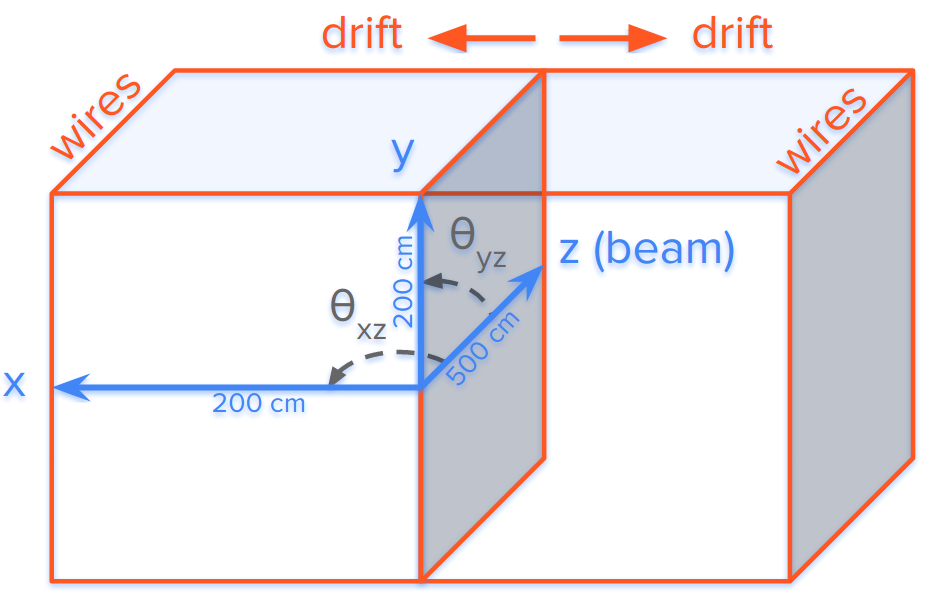
\includegraphics[width =\largefigwidth]{Figures/SBND_geometry.png}
    \caption{The SBND coordinate system showing the definition of the $\theta_{XZ}$ and $\theta_{YZ}$ angles.}
    \label{fig:my_label}
\end{figure}

Expect the hit resolution to be poor when showers are directed in the drift direction. There will be a large pulse train on just a few wires which means the hit reconstruction will suffer. 
\begin{figure}
    \centering
    \fbox{
    \begin{minipage}{0.8\textwidth}
    Reco efficiency vs XZ angle (Y is fixed at 0m).
    Don't think I understand why there is a local peak at +- 90ish degrees, I would have expected the performance to be at its worst for these cases. Otherwise looks sensible I think. 
    \end{minipage}
    }
    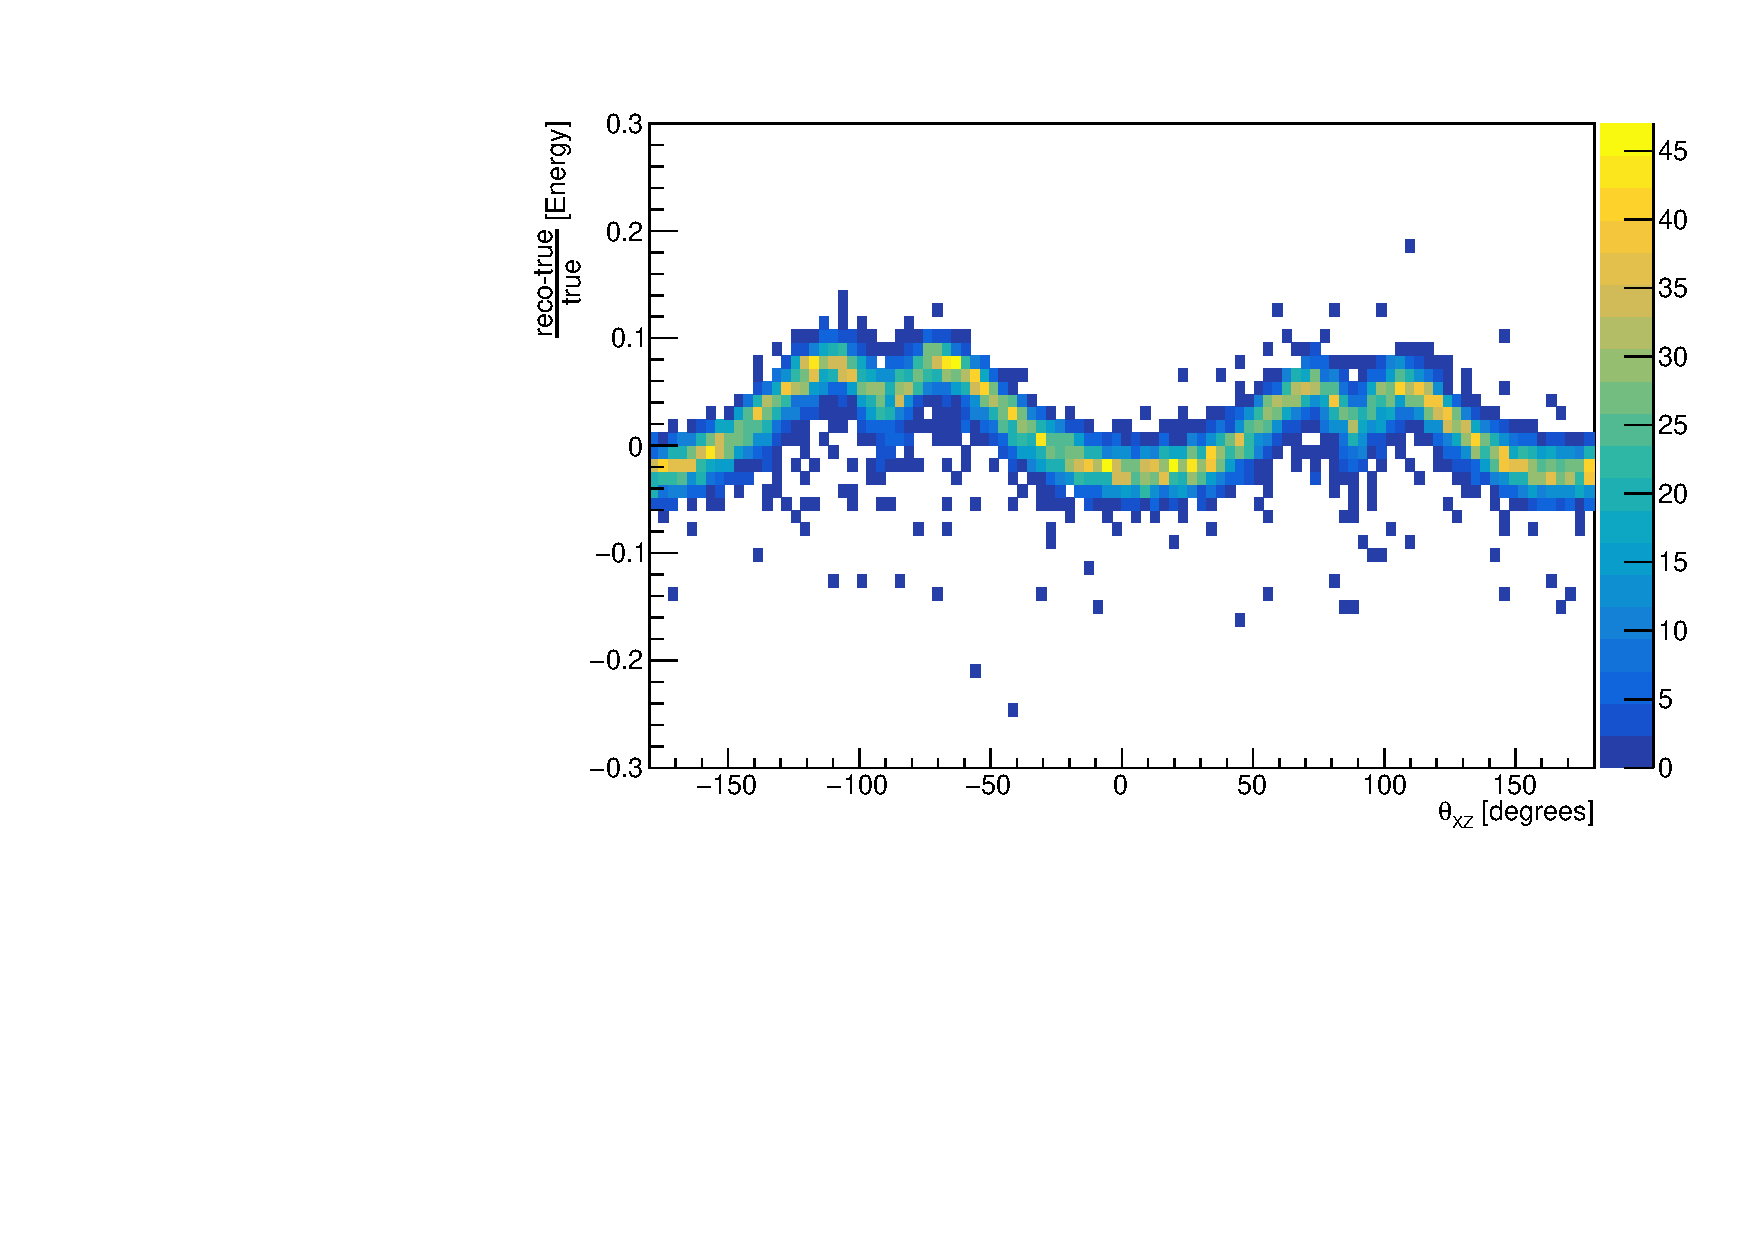
\includegraphics[width = \largefigwidth]{Figures/frac_res_vs_thetaXZ_cheating_electron_vertex_plane2.pdf}
    \caption{The fractional resolution of the shower energy from an $\electron \pi^+$ vertex sample vs the angle of the electron in the X-Z plane (i.e. Y is fixed at 0). Reconstruction performed from the hits collected by plane 2.}
    \label{fig:my_label}
\end{figure}

\begin{figure}
    \centering
    \fbox{Reco efficiency vs YZ angle (X is fixed at 1m)}
    \caption{Caption}
    \label{fig:my_label}
\end{figure}

\begin{figure}
    \centering
    \fbox{Reco efficiency vs true deposited energy}
    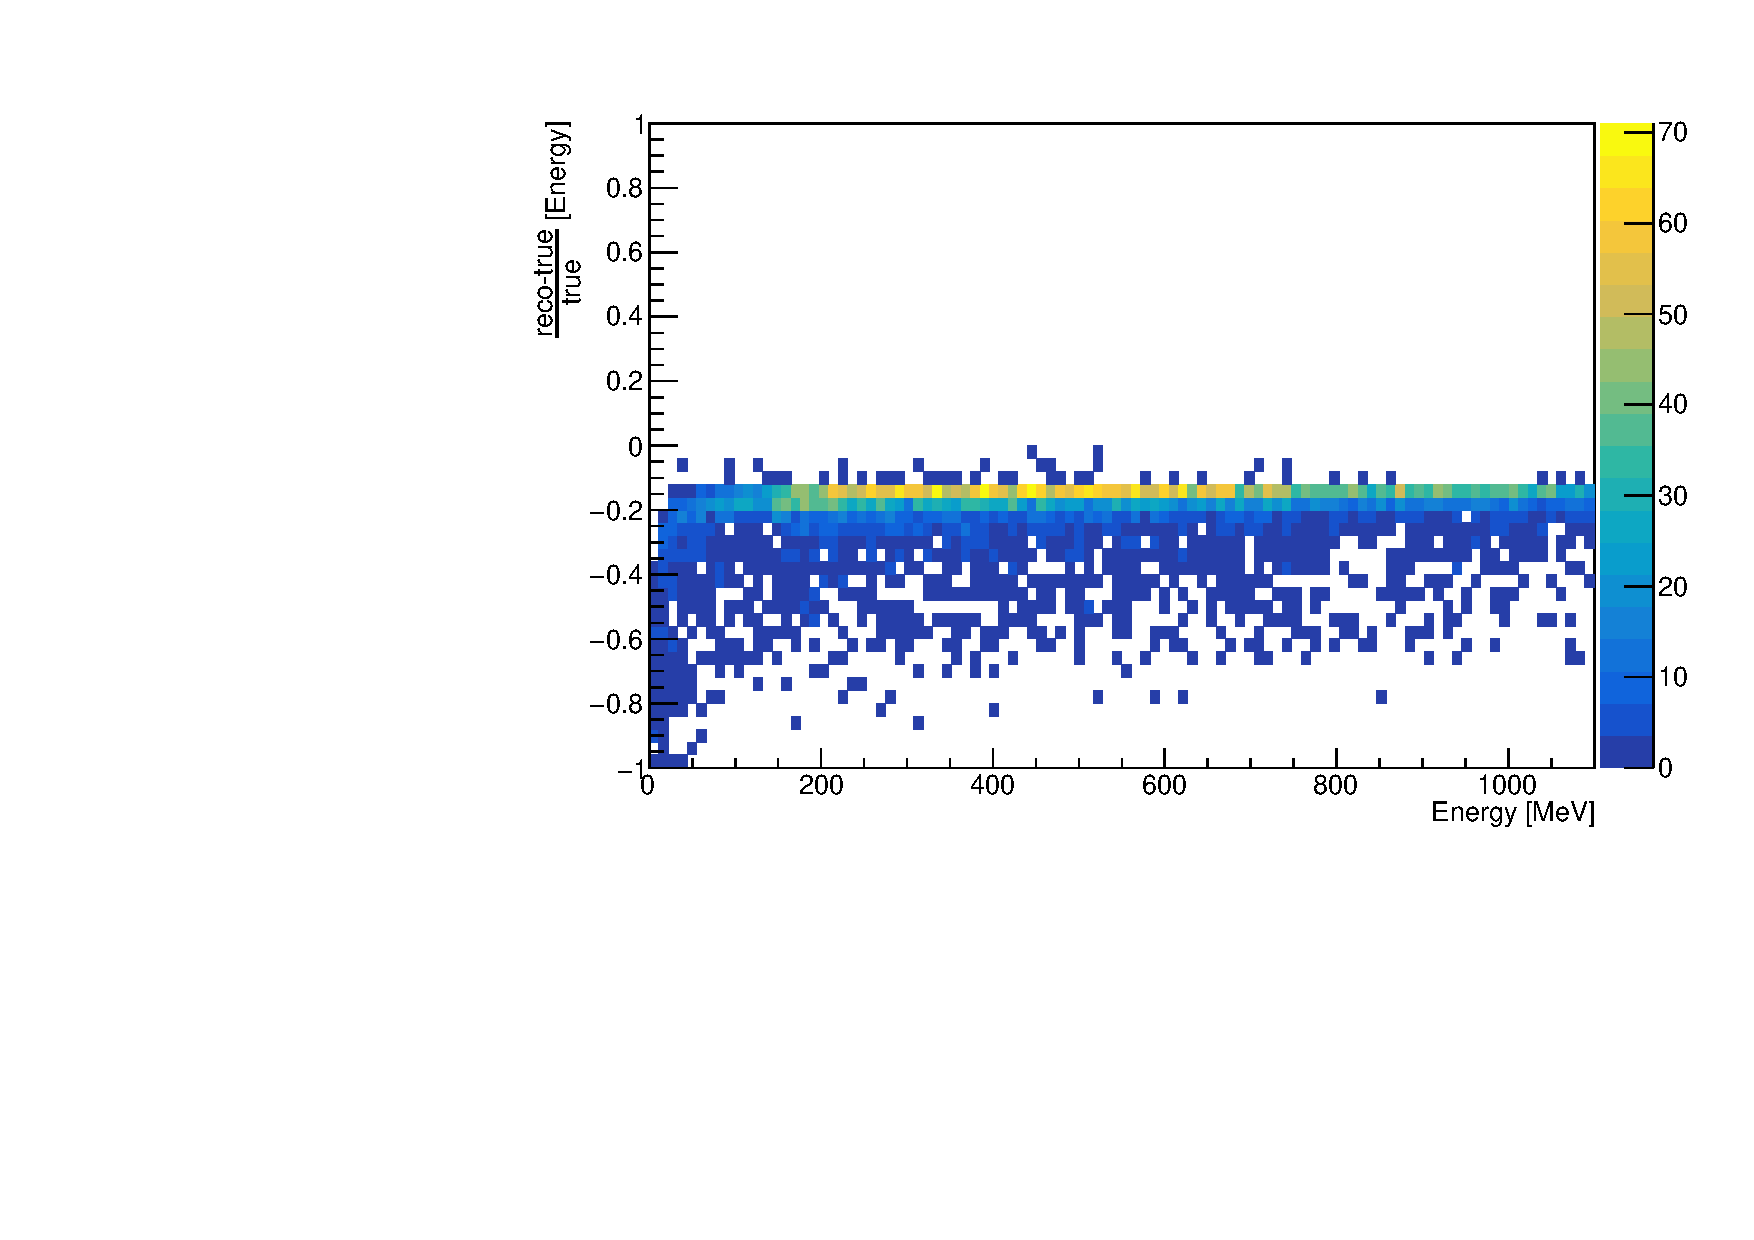
\includegraphics[width = \largefigwidth]{Figures/frac_res_vs_hit_energy_electron_vertex_plane2.pdf}
    \caption{The fractional resolution of the shower energy from an $\electron \pi^+$ vertex sample vs the sum of the true hit energy. Reconstruction performed from the hits collected by plane 2. The resolution is largely consistent across all energies with maybe a minor dip in performance for low energy showers.}
    \label{fig:my_label}
\end{figure}

\begin{figure}
    \centering
    \fbox{Cheated Reco efficiency vs true deposited energy}
    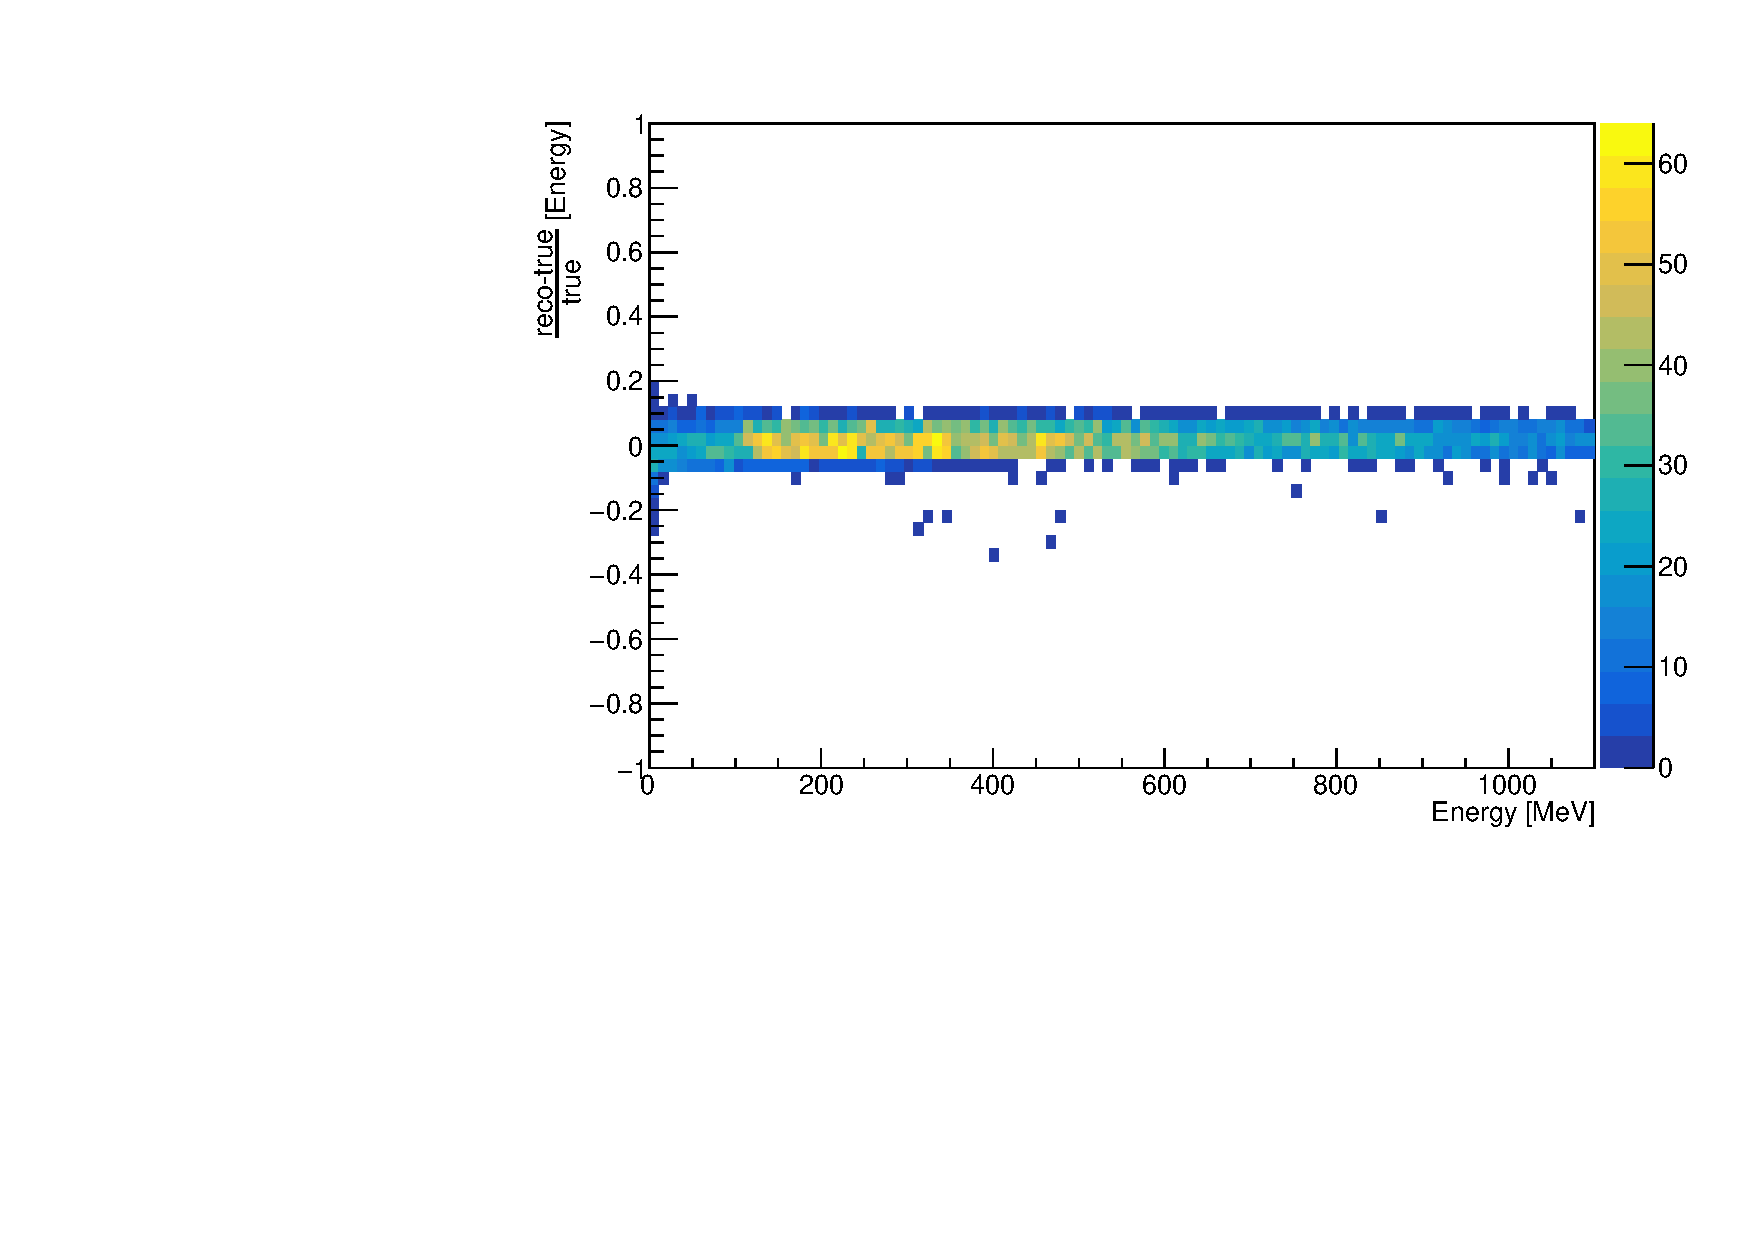
\includegraphics[width = \largefigwidth]{Figures/frac_res_vs_hit_energy_cheating_electron_vertex_plane2.pdf}
    \caption{The fractional resolution of the shower energy from an $\electron \pi^+$ vertex sample vs the sum of the true hit energy. Using cheated pattern recognition with the reconstruction performed from the hits collected by plane 2. The resolution is largely consistent across all energies with maybe a minor dip in performance for low energy showers.}
    \label{fig:my_label}
\end{figure}

\begin{figure}
    \centering
    \fbox{Fractional resolution of \electron $\pi^+$ with lower (no?) hit thresholding.}
    \caption{Caption}
    \label{fig:my_label}
\end{figure}

\begin{figure}
    \centering
    \fbox{Validation with some sort of low energy sample (supernova neutrinos?)}
    \caption{Caption}
    \label{fig:my_label}
\end{figure}



